\documentclass{article}
 
\usepackage{amsmath}
\usepackage{amssymb}
\usepackage{graphicx}
\usepackage{verbatim}
\usepackage{enumerate}
\usepackage[utf8]{inputenc}
\newcommand{\beq}{\begin{equation}}
\newcommand{\eeq}{\end{equation}}
%\verbatiminput{verb.txt}
\begin{document}
\title{Mandatory Assignment I}
\author{Shafa Aria}
\maketitle
\begin{enumerate}
\item{I}
For the first assignment we would look at the various non-circular duct solutions and compute them in FEniCS with higher order degrees. We did this for three non-circular ducts: Ellipse, Equilateral triangle and an eccentric annulus.\\

for the Ellipse the results are as follows:
\begin{verbatim}
h=2.44E-01 E=6.36E-02 r=1.70
h=1.18E-01 E=1.65E-02 r=1.86
h=5.72E-02 E=4.14E-03 r=1.90
h=2.80E-02 E=1.03E-03 r=1.94
\end{verbatim}
We see that it converges towards 2. The figures are as follows:\\
\hspace{-4cm}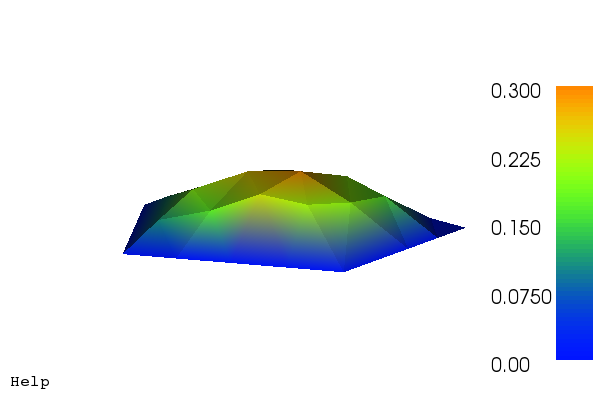
\includegraphics[scale=0.3]{dolfin_plot_0.png}
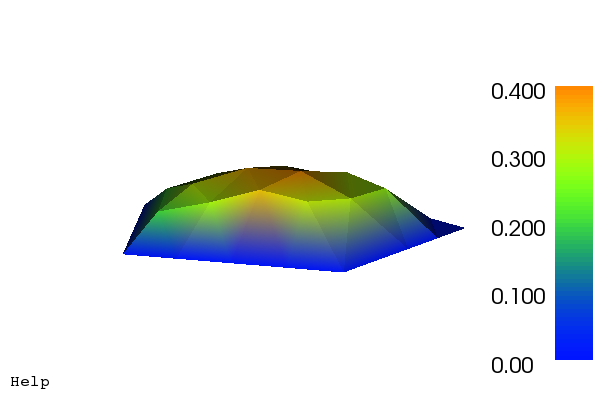
\includegraphics[scale=0.3]{dolfin_plot_1.png}\\
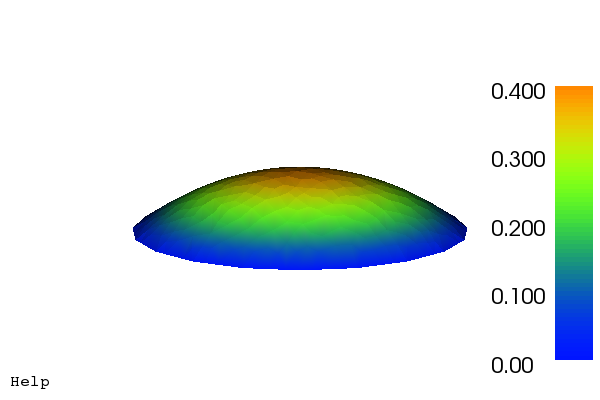
\includegraphics[scale=0.3]{dolfin_plot_2.png}
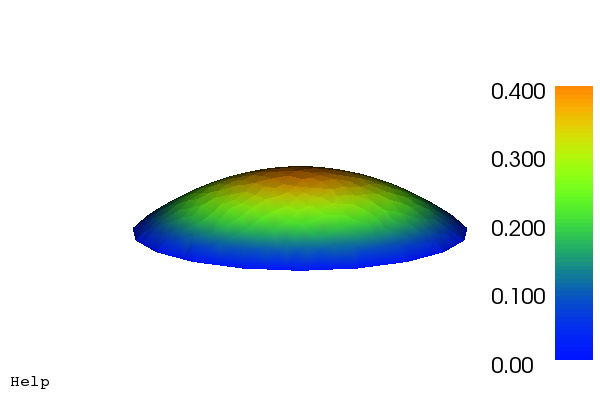
\includegraphics[scale=0.3]{dolfin_plot_3.png}\\
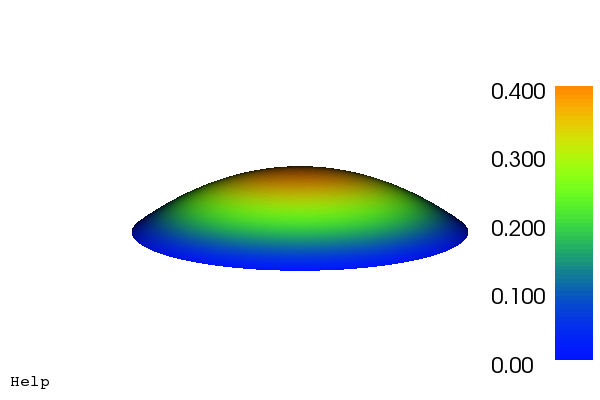
\includegraphics[scale=0.3]{dolfin_plot_4.png}
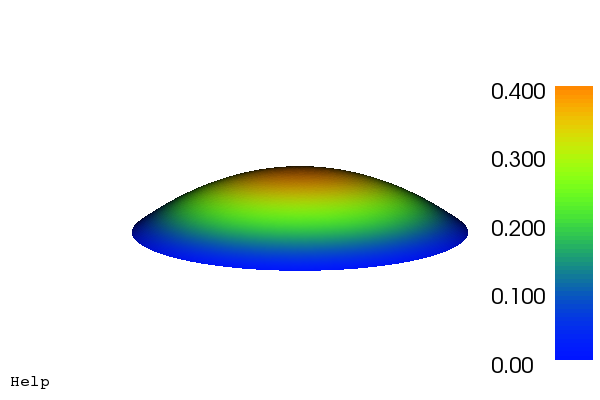
\includegraphics[scale=0.3]{dolfin_plot_5.png}\\
Where I have only included the figures for $N=5,20,80$ as we can see the mesh gets finer as we increase the mesh points.\\

For the equilateral triangle and the eccentric annulus I was only able to come up with the numerical solutions. For some reason the exact solution could not be implemented and I could not find the reason for why not. Thus I was unable to calculate the $E$ and $r$.
For the eccentric annulus: 
\begin{verbatim}
h=2.38E-01 E=NAN r=nan
h=1.19E-01 E=NAN r=nan
h=5.78E-02 E=NAN r=nan
h=2.76E-02 E=NAN r=nan
\end{verbatim}
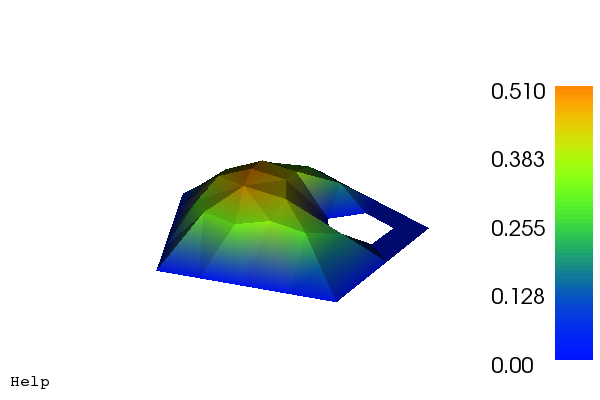
\includegraphics[scale=0.3]{dolfin_plot_6.png}
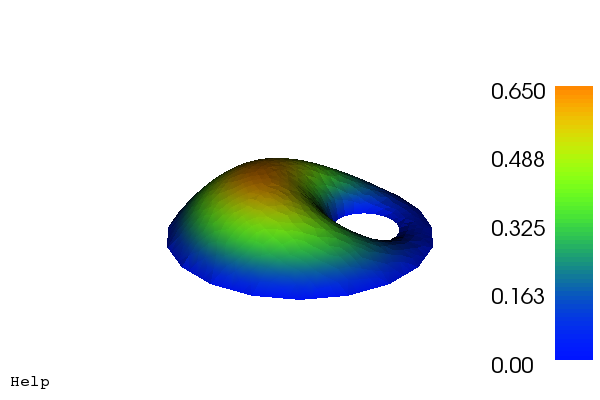
\includegraphics[scale=0.3]{dolfin_plot_7.png}\\
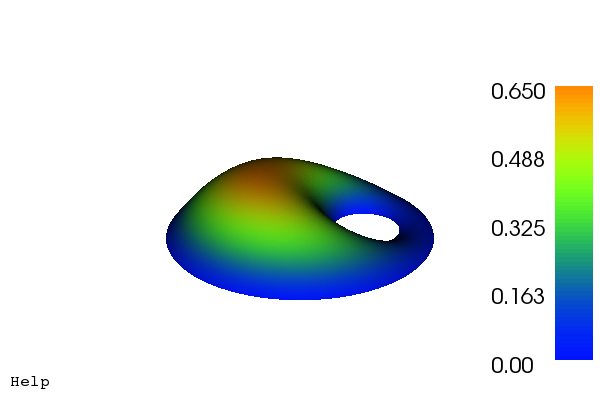
\includegraphics[scale=0.3]{dolfin_plot_8.png}\\

For the triangle the problem was the inversion of the coordinates. For some reason my FEniCS version would not allow me to insert the $z=h-x$ into the expression. Thus I could not inverse the exact solution. 
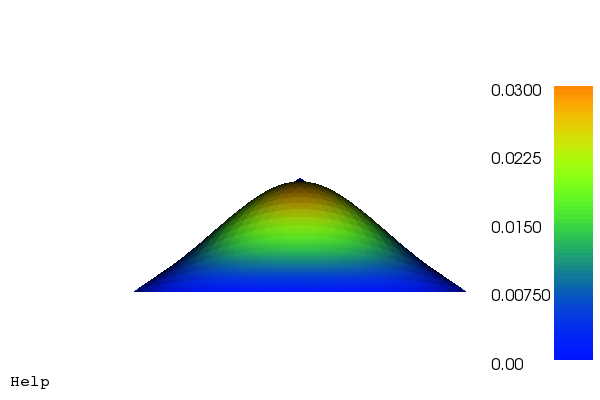
\includegraphics[scale=0.3]{dolfin_plot_9.png}
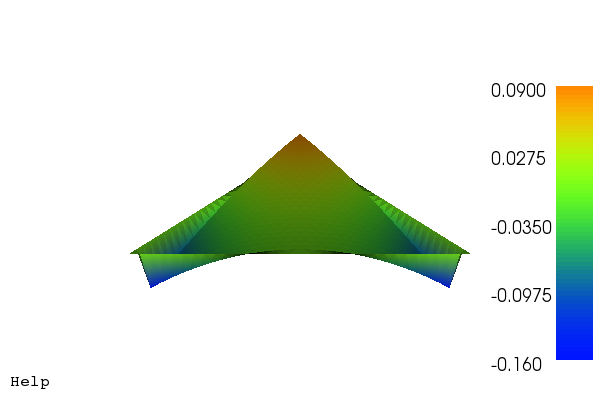
\includegraphics[scale=0.3]{dolfin_plot_10.png}\\
\item{IV}
For the last exercise I generated the mesh in gmsh and converted it into an xml file and imported into the python code as was shown in the lecture notes.\\
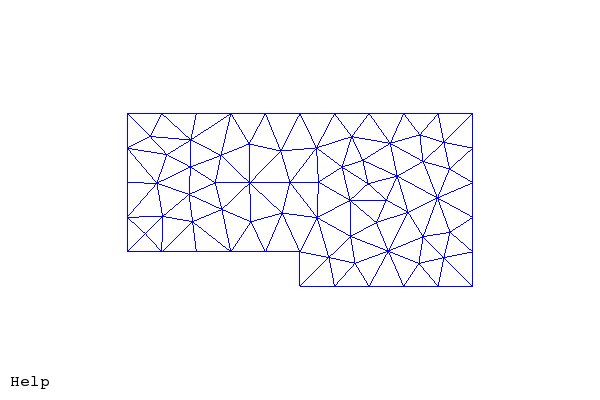
\includegraphics[scale=0.3]{dolfin_plot_11.png}\\
I solved the Stoke's equation and got the following plot in FEniCS\\
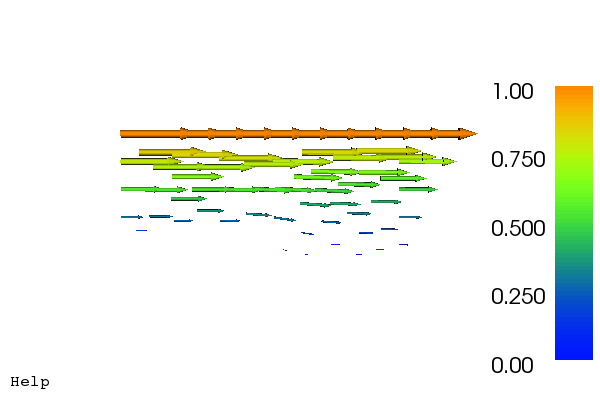
\includegraphics[scale=0.3]{dolfin_plot_12.png}\\
Where it shows the flow through down the step. Unfortunately I was yet again not able to plot the streamfunction so I could use paraview to look closer at the vortex.\\
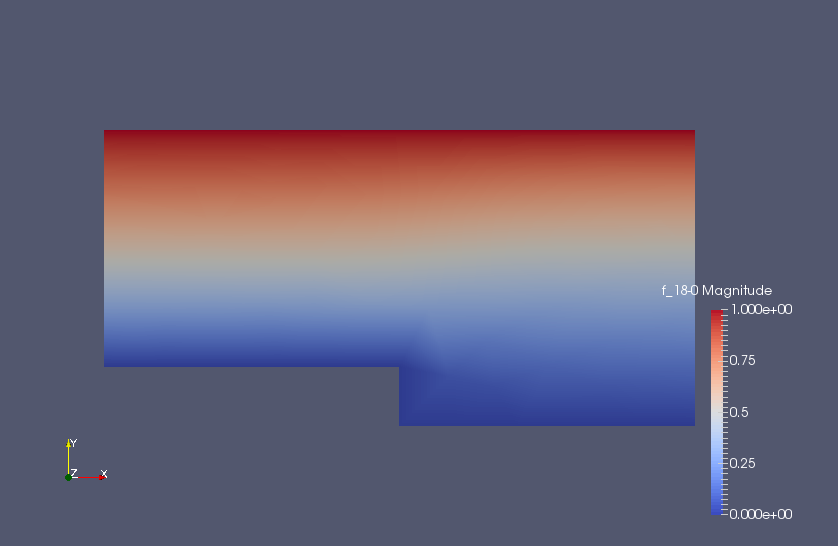
\includegraphics[scale=0.3]{paraview_plot1.png}\\

\item{CODE: ELLIPSE}
\begin{verbatim}
from dolfin import *
from numpy import cosh, cos
set_log_active(False)
from math import log as ln
from mshr import *

dpdx = Constant(-0.01)
mu = Constant(0.01)
a = 2
b = 1
c = 0
# Much faster C++ version
ue_code = '''
class U : public Expression
{
  public:

    double a, b, mu, dpdx;

  void eval(Array<double>& values, const Array<double>& x) const
    {
      double u = 0.;
      double factor = 1.0/(2*mu)*(-dpdx)*(a*a*b*b)/(a*a + b*b);
      u = 1.0-(x[0]*x[0])/(a*a) - (x[1]*x[1])/(b*b);
      values[0] = u*factor;      
    }
};'''

# assigning the parametres into the c++ code?
u_c = Expression(ue_code)
u_c.a = float(a); u_c.b = float(b)
u_c.mu = float(mu(0)); u_c.dpdx = float(dpdx(0))

mesh = generate_mesh(Ellipse(Point(c),a ,b, 32), 32)

def main(N, degree=1):
  mesh = generate_mesh(Ellipse(Point(c),a ,b, N), N)
  V = FunctionSpace(mesh, 'CG', degree)
  u = TrialFunction(V)
  v = TestFunction(V)
  F = inner(grad(u), grad(v))*dx + 1/mu*dpdx*v*dx
  bc = DirichletBC(V, Constant(0), DomainBoundary())
  u_ = Function(V)
  solve(lhs(F) == rhs(F), u_, bcs=bc)

  #u_e = interpolate(u_exact(), V)
  u_e = interpolate(u_c, V)
  bc.apply(u_e.vector())
  u_error = errornorm(u_e, u_, degree_rise=0)

  if N==5 or N==20 or N==80:
    plot(u_, title="Numerical")
    plot(u_e, title="Exact")
    interactive()
  return u_error, mesh.hmin()

E = []; h = []; degree = 3
for n in [5, 10, 20, 40, 80]:
  ei, hi = main(n, degree=degree)
  E.append(ei)
  h.append(hi)

for i in range(1, len(E)):   
    r = ln(E[i]/E[i-1])/ln(h[i]/h[i-1])
    print "h=%2.2E E=%2.2E r=%.2f" %(h[i], E[i], r)

\end{verbatim}
\item{CODE: ECCENTRIC ANNULUS}
\begin{verbatim}
from dolfin import *
from numpy import log, sqrt, cosh, sinh, cos, sin
set_log_active(False)
from mshr import *

dpdx = Constant(-0.01)
mu = Constant(0.01)
a = 2
b = 0.5
c = 1

F = (a*a - b*b + c*c)/(2*c)
M = sqrt((F*F - a*a))
alpha = 0.5*log((F + M)/(F - M))
beta = 0.5 * log((F - c + M)/(F - c - M))

# Much faster C++ version
ue_code = '''
class U : public Expression
{
  public:

    double a, b, c, mu, dpdx, F, M, alpha, beta;
  void eval(Array<double>& values, const Array<double>& x) const
    {
      double Q = 0.;
      double factor = DOLFIN_PI/(8*mu)*(-dpdx);
      for (std::size_t n=1; n<600; n++)
        Q += (n * exp(-n*(beta + alpha)))/(sinh(n*beta - n*alpha));

      values[0] = factor * (pow(a,4) - pow(b,4) - \
      (4 * c*c * M*M)/(beta - alpha) - 8 * c*c * M*M * Q);      
    }
};'''

u_c = Expression(ue_code)
u_c.a = float(a); u_c.b = float(b)
u_c.mu = float(mu(0)); u_c.dpdx = float(dpdx(0))
u_c.c = float(c); u_c.F = float(F); u_c.M = float(M)
u_c.alpha = float(alpha); u_c.beta = float(beta)

def main(N, degree=1):
    mesh = generate_mesh(Circle(Point(0.0,0.0), a, N) - Circle(Point(a-c), b, N), N)
    V = FunctionSpace(mesh, 'CG', degree)
    u = TrialFunction(V)
    v = TestFunction(V)
    F = inner(grad(u), grad(v))*dx + 1/mu*dpdx*v*dx
    bc = DirichletBC(V, Constant(0), DomainBoundary())
    u_ = Function(V)
    solve(lhs(F) == rhs(F), u_, bcs=bc)

    # u_e = interpolate(u_exact(), V)
    u_e = interpolate(u_c, V)
    bc.apply(u_e.vector())
    u_error = errornorm(u_e, u_, degree_rise=0)

    if N==5 or N==20 or N==80:
      plot(u_,title="Numerical")
      plot(u_e,title="Exact")
      interactive()
    return u_error, mesh.hmin()

E = []; h = []; degree = 2
for n in [5, 10, 20, 40, 80]:
    ei, hi = main(n, degree=degree)
    E.append(ei)
    h.append(hi)

from math import log as ln
for i in range(1, len(E)):
    r = ln(E[i]/E[i-1])/ln(h[i]/h[i-1])
    print "h=%2.2E E=%2.2E r=%.2f" %(h[i], E[i], r)
\end{verbatim}

\item{CODE:TRIANGLE}
\begin{verbatim}
from dolfin import *
from numpy import cosh, cos
set_log_active(False)
from math import log as ln
from mshr import *

dpdx = Constant(-0.01)
mu = Constant(0.01)
a = 2
b = 1
c = 0
# Much faster C++ version
ue_code = '''
class U : public Expression
{
  public:

    double a, b, mu, dpdx;

  void eval(Array<double>& values, const Array<double>& x) const
    {
      double u = 0.;
      double factor = -dpdx * 1/(2*sqrt(3)*a*mu);
      u = (x[1] - 0.5*a*sqrt(3))*(3*x[0]*x[0] - x[1]*x[1]);
      values[0] = u*factor;      
    }
};'''

# assigning the parametres into the c++ code?
u_c = Expression(ue_code)
u_c.a = float(a); u_c.b = float(b)
u_c.mu = float(mu(0)); u_c.dpdx = float(dpdx(0))

def main(N, degree=1):
  mesh = Mesh("triangle_gmsh.xml")
  V = FunctionSpace(mesh, 'CG', degree)
  u = TrialFunction(V)
  v = TestFunction(V)
  F = inner(grad(u), grad(v))*dx + 1/mu*dpdx*v*dx
  bc = DirichletBC(V, Constant(0), DomainBoundary())
  u_ = Function(V)
  solve(lhs(F) == rhs(F), u_, bcs=bc)

  #u_e = interpolate(u_exact(), V)
  u_e = interpolate(u_c, V)
  bc.apply(u_e.vector())
  u_error = errornorm(u_e, u_, degree_rise=0)

  plot(u_, title="Numerical")
  plot(u_e, title="Exact")
  interactive()
  return u_error, mesh.hmin()

E = []; h = []; degree = 4
for n in [5, 10, 20, 40, 80]:
  ei, hi = main(n, degree=degree)
  E.append(ei)
  h.append(hi)

for i in range(1, len(E)):

  r = ln(E[i]/E[i-1])/ln(h[i]/h[i-1])
  print "h=%2.2E E=%2.2E r=%.2f" %(h[i], E[i], r)
\end{verbatim}

\newpage


\item{CODE: STOKE'S FLOW}
\begin{verbatim}
from dolfin import *
import numpy
#from mshr import *

mu = Constant(1.0)

mesh = Mesh("step.xml")


V = VectorFunctionSpace(mesh, 'CG', 2)
Q = FunctionSpace(mesh, 'CG', 1)
VQ = MixedFunctionSpace([V,Q])
u, p = TrialFunctions(VQ)
v, q = TestFunctions(VQ)
F = mu*inner(grad(v), grad(u))*dx - inner(div(v), p)*dx - \
			inner(q, div(u))*dx +Constant(0)*q*dx
s0 = AutoSubDomain(lambda x, on_bnd: x[1]>0.5-1e-8)
Top = DirichletBC(VQ.sub(0), (1,0),s0)
s1 = AutoSubDomain(lambda x, on_bnd: x[1]<1e-8)
Bottom1 = DirichletBC(VQ.sub(0), (0,0), s1)

def b_boundary(x):
	return x[1]< 0.1+DOLFIN_EPS and x[0]<0.5+DOLFIN_EPS

Bottom2 = DirichletBC(VQ.sub(0), (0,0), b_boundary)

up_ = Function(VQ)
bcs = [Top,Bottom1,Bottom2]
solve(lhs(F)==rhs(F), up_, bcs=bcs)
u_, p_ = up_.split()
#plot(u_,interactive=True)
#f = File("solution.pvd")
#f << u_

#streamfunction:
q = TestFunction(V)
psi = TrialFunction(V)
n = FacetNormal(mesh)
F = inner(grad(q), grad(psi))*dx \
- inner(q, (u[1].dx(0) - u[0].dx(1)))*dx \
+ q*(n[1]*u[0] - n[0]*u[1])*ds +Constant(0)*q*dx
solve(lhs(F)=rhs(F),U,bcs=bcs)

\end{verbatim}

\end{enumerate}
\end{document}
